% !TEX root = ../../thesis.tex

\section{Figures \& Tables}%
\label{sec:basics-figures_and_tables}%

\subsection*{Figures}%
Figures are typically made up of a \verb|figure| environment, a \verb|\centering| command to keep the content aligned in the middle of the page, an \verb|\includegraphics| command to insert the image itself, a \verb|\caption| command to insert a caption, and a \verb|\label| command to give it a referenceable name, which we will look at later.

Figure~\ref{fig:basics-skyrim_book} shows how to insert a single figure with a caption.
The image is inserted using the \verb|\includegraphics| command, where its \verb|width| option is used to size the image relative to the text's maximum width.
A caption is also added and placed below the image with the \verb|\caption| command, and \verb|\label| is used to provide an anchor that we can reference in text, as the start of this paragraph did.
The position of the image is controlled by both its literal position in the \LaTeX{} source as well as an optional argument to the \verb|\figure| environment.
Placement of figures in \LaTeX{} can be tricky and they can often end up where you don't want them to!

% Note how this is wrapped in the 'figure' environment. The "!htbp" is a positioning hint. Have a search online for more details.
\begin{figure}[!htbp]
  % This ensures that the image is centered on the page. You almost always want this.
  \centering
  % This is now we include graphics. The argument in the square brackets defines the image width as a 0-1 percentage of the text's width.
  % You can also use direct sizes here, too, but this is most common. The actual image is specified WITHOUT its extension.
  % Remember in the parent basics.tex file, we set graphics path as "\graphicspath{{chapters/basics/figures/}}"?
  % The images are relative to that. As other chapters refined graphicspath, they become relative to that path, and so on.
  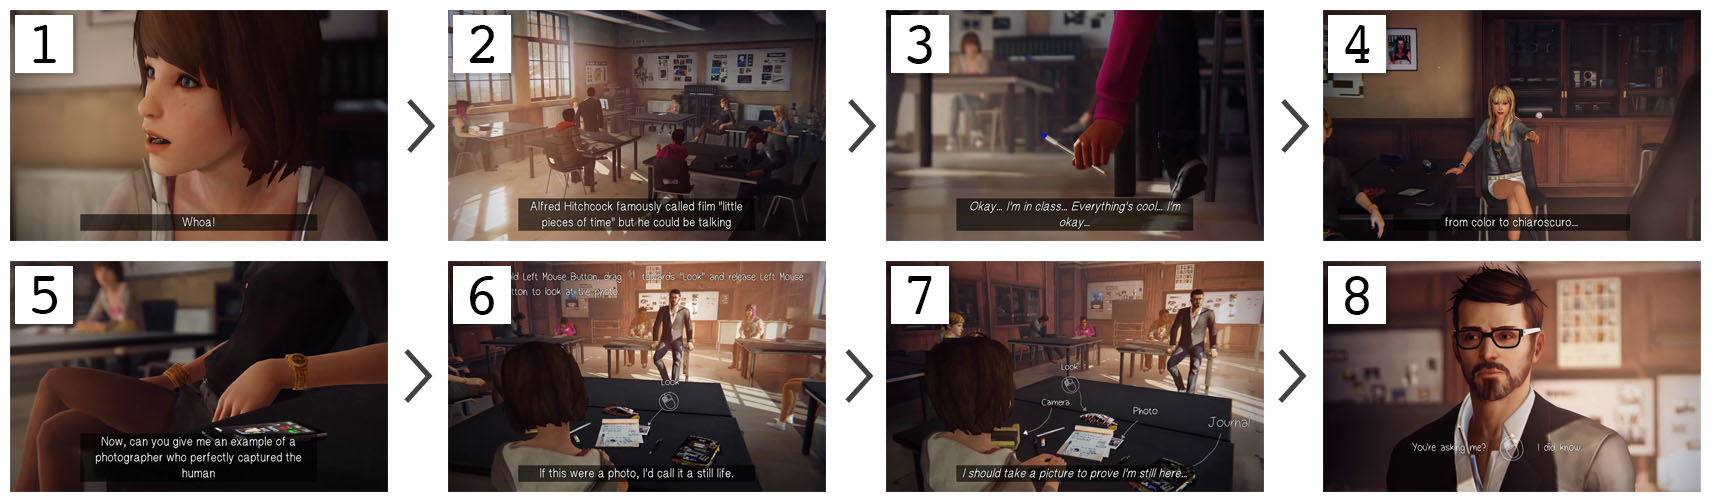
\includegraphics[width=1.0\textwidth]{lis-overview}
  % This caption appears below the image. If you want it above, simply move the line up above \includegraphics.
  \caption{A high-level overview of the \textit{Life is Strange} sequence. 1.\ Max wakes up in class. 2.\ A lecture is taking place. 3.\ Stella drops her pen. 4.\ Taylor bullies Kate. 5.\ Victoria's phone vibrates. 6.\ Max's desk interactions. 7.\ Max's camera usage prompt. 8.\ Max's questioning for disturbing class.}%
  % This defines a label that we can \ref{} later, which we will be doing!
  \label{fig:basics-skyrim_book}
\end{figure}

Figure~\ref{fig:basics-obra} shows how to stack multiple images together in one figure either horizontally or vertically.
We can even reference its parts like Figure~\ref{fig:basics-obra_1} and Figure~\ref{fig:basics-obra_2}.
In this template, this is achieved with the \verb|subfig| package and its \verb|\subfloat| command.

% Notice how there are TWO labels here. This lets us reference Figure X.A, X.B separately.
\begin{figure}[!htbp]
  \centering
  
  % Notice how we're using the \subfloat command to insert a caption, then \includegraphics and \label are used inside its brackets.
  \subfloat[Entering Part 4 of Chapter IV by interacting with Bun-Lan Lin's body. Parts 1, 2, and 3 unavailable at this point.]{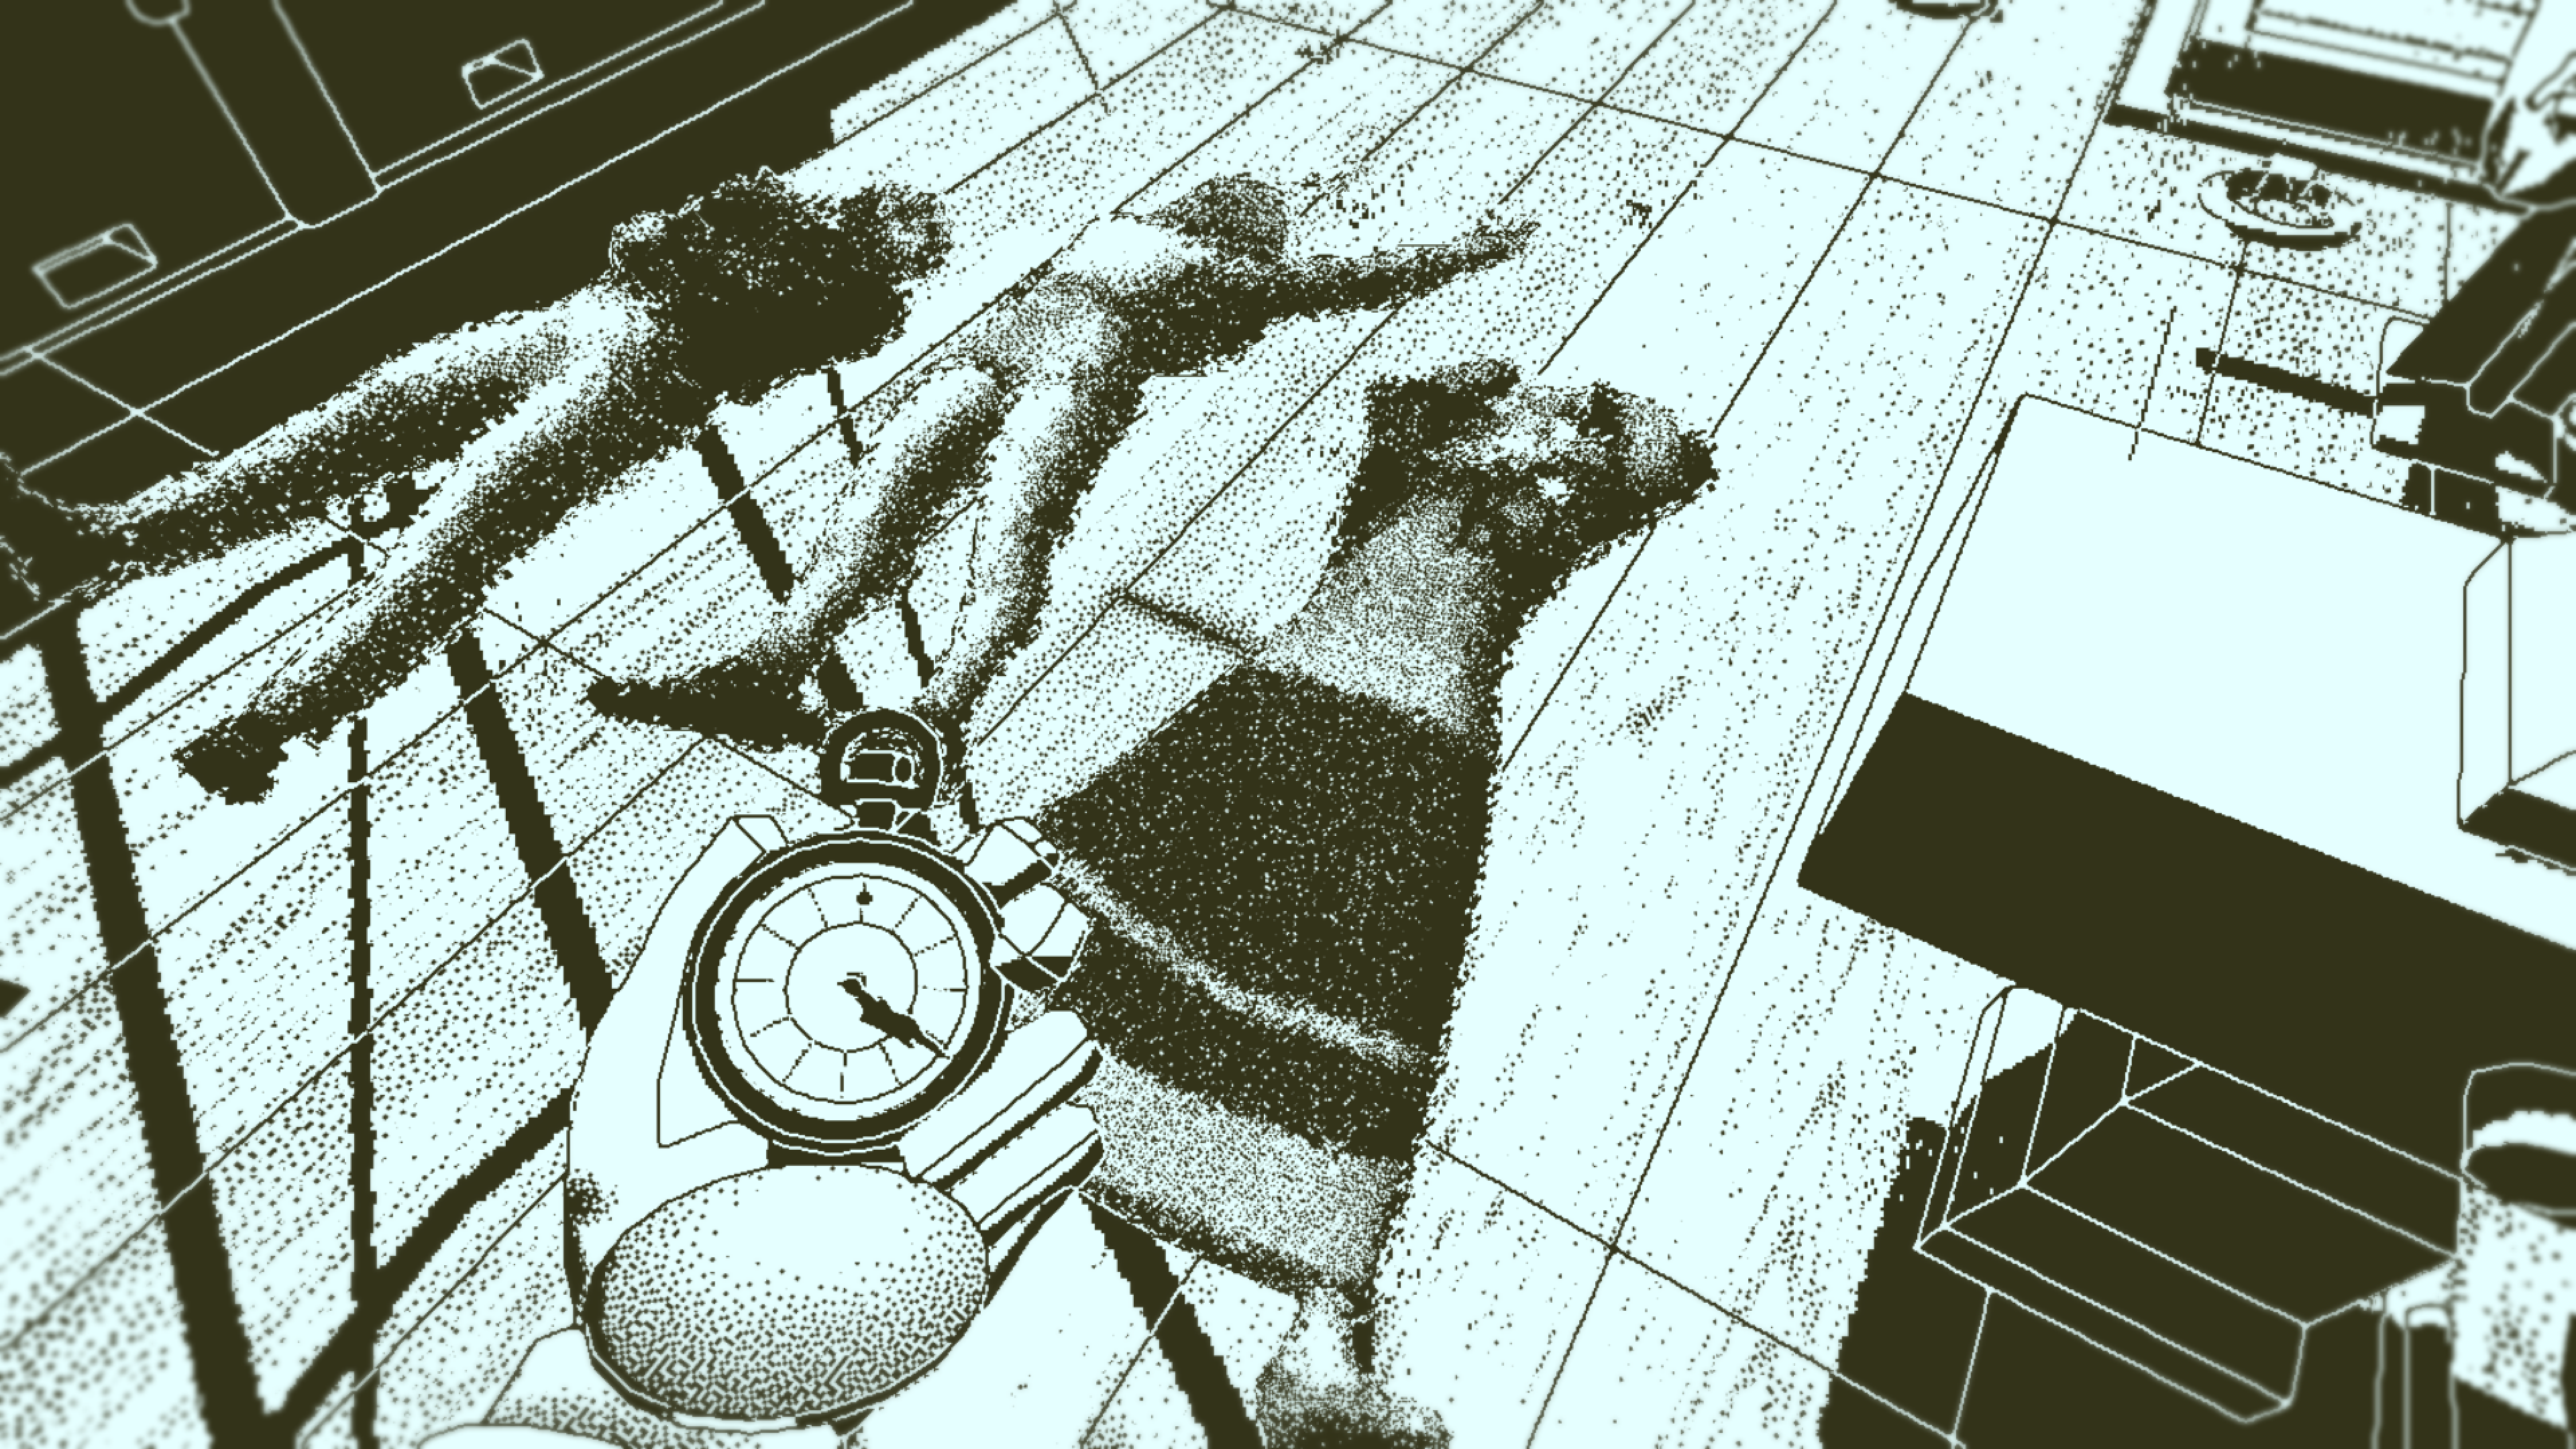
\includegraphics[width=.48\textwidth]{obra-1}\label{fig:basics-obra_1}}
  % This helps with spacing between horizontal images.
  \quad
  % Notice how the size is less than 50% (0.48 in this case). This is so that there's room around each image for spacing.
  % If you just used 50%, they would stack vertically instead of horizontally.
  \subfloat[Entering Part 2 from within Part 4 by locating and interacting with Patrick O'Hagan's body.]{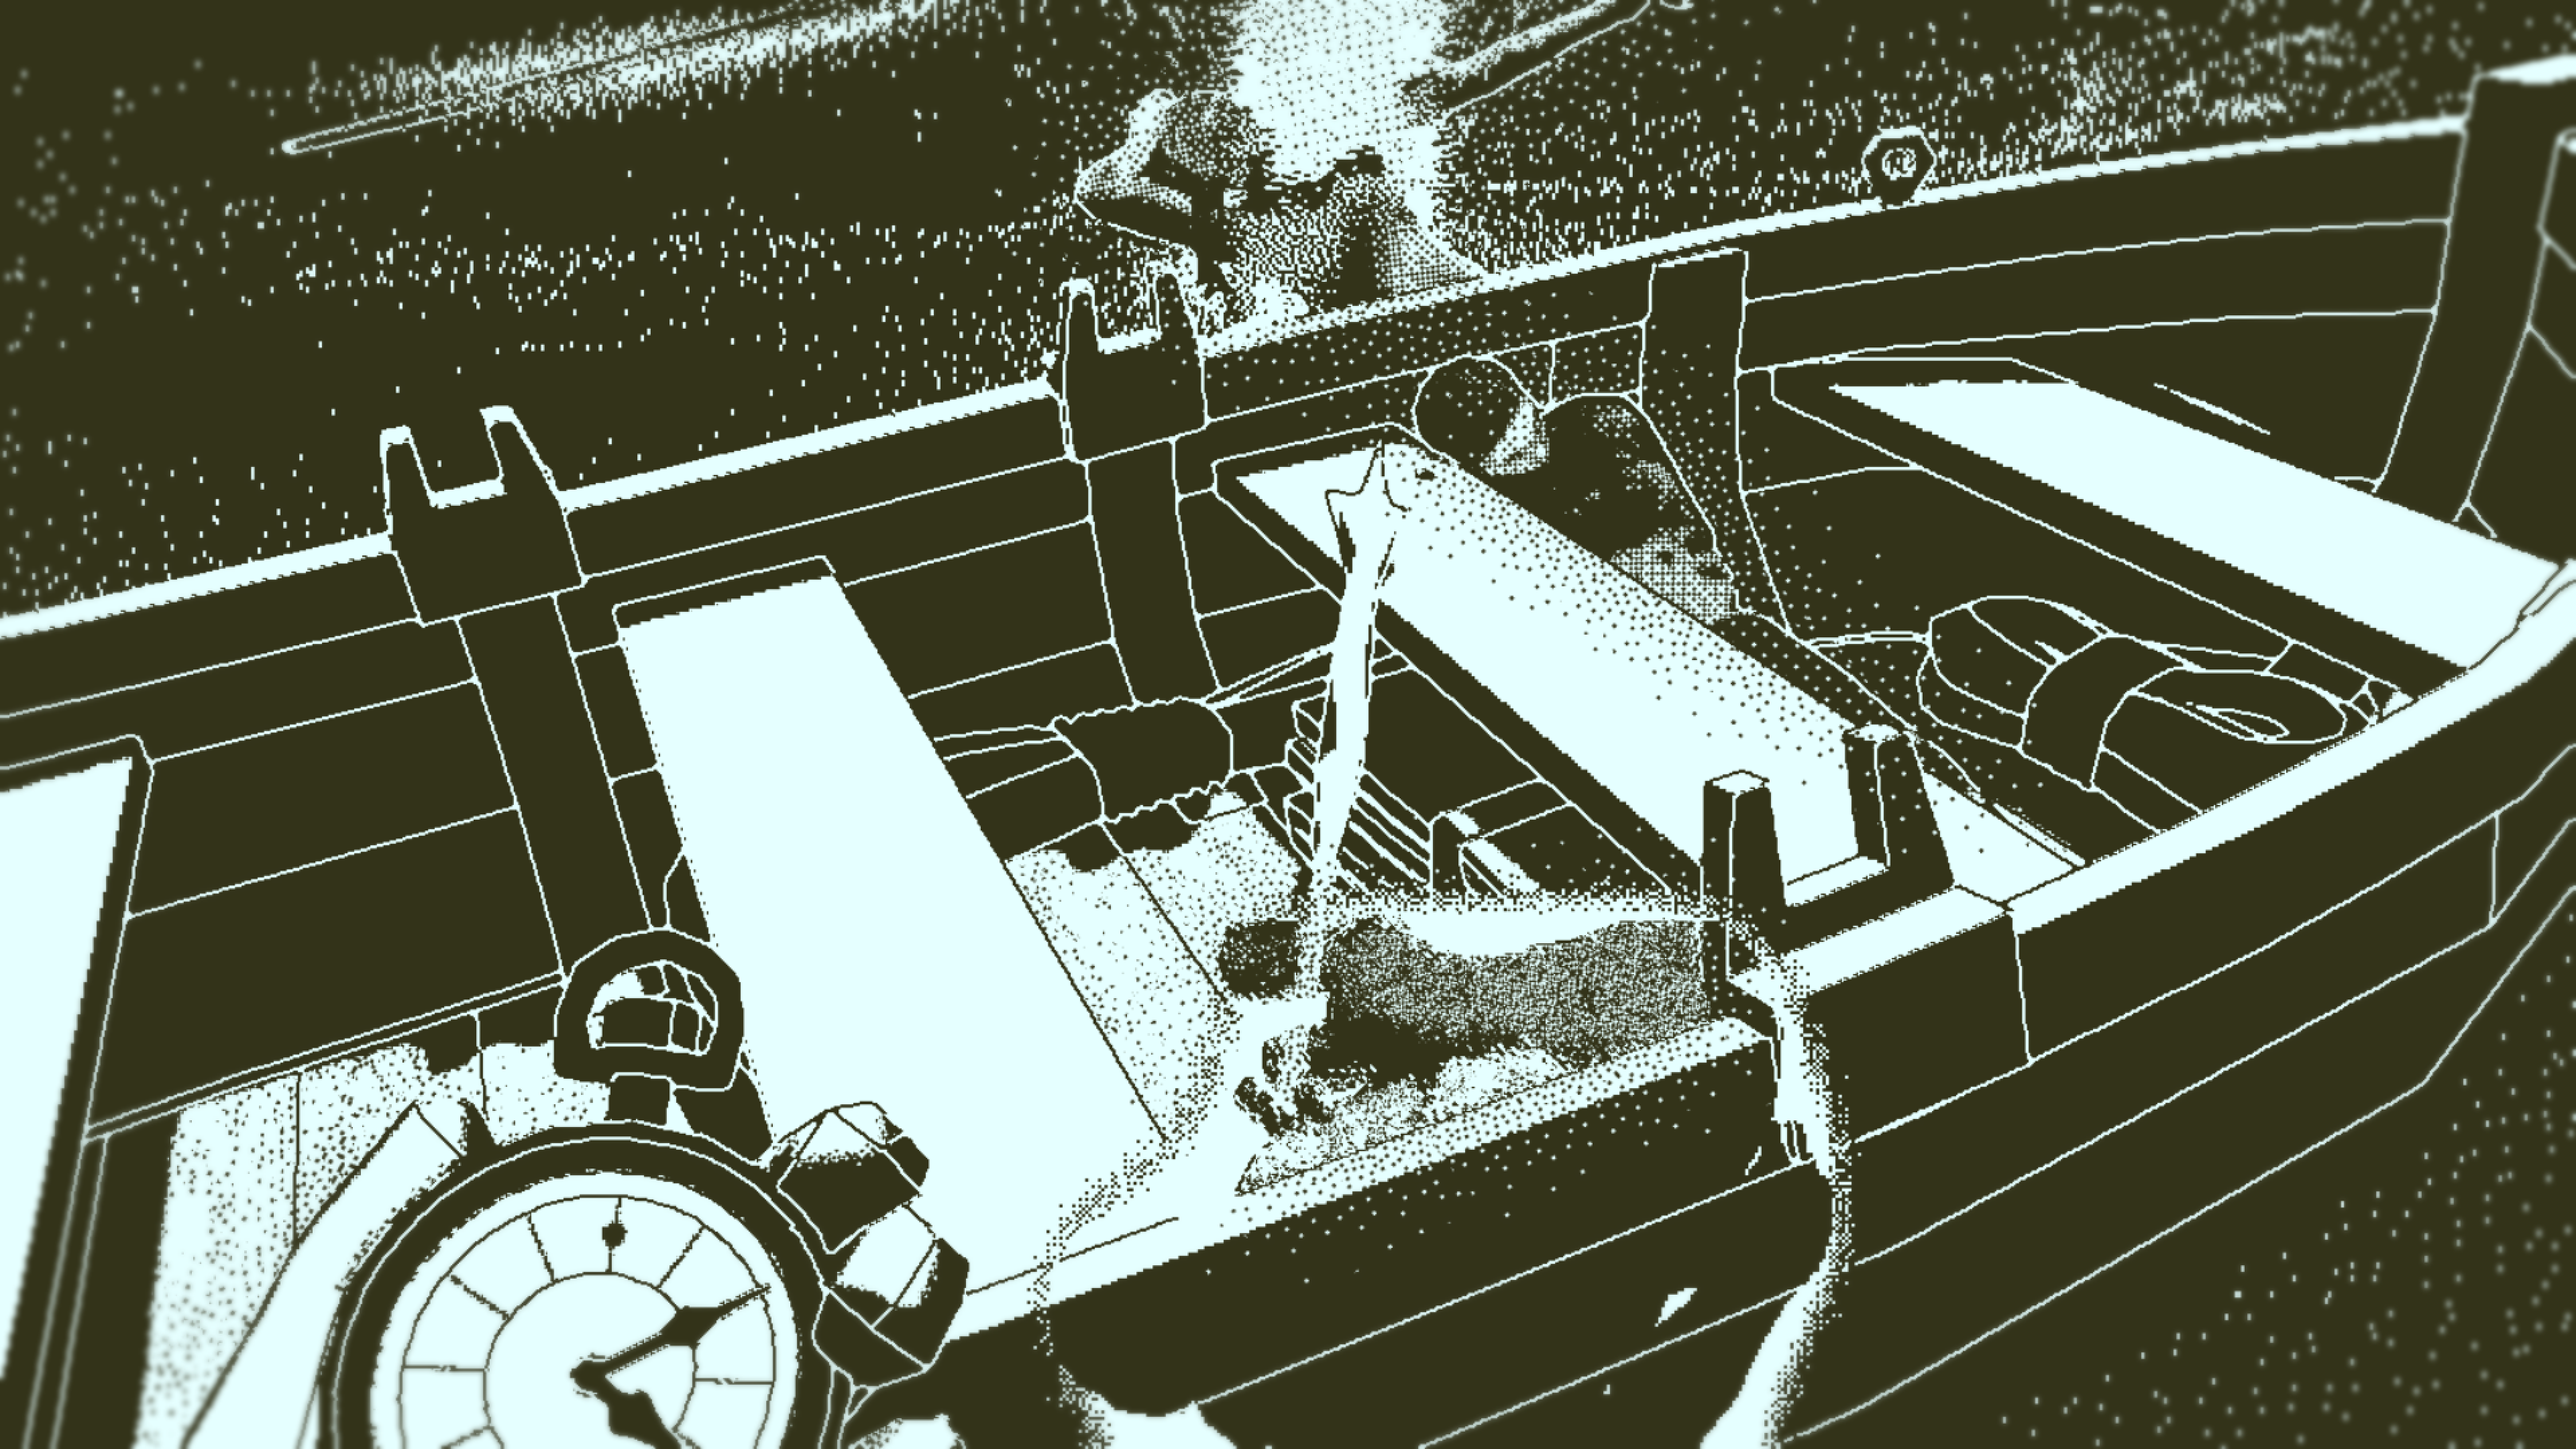
\includegraphics[width=.48\textwidth]{obra-2}\label{fig:basics-obra_2}}
  \caption{A player in \textit{Return of the Obra Dinn} entering into Part 4 of Chapter IV by interacting with Bun-Lan Lin's body on the main deck. From Part 4, they discover Patrick O'Hagan's body, which can take them to Part 2 of the same Chapter.}

  \label{fig:basics-obra}
\end{figure}

\subsection*{Tables}%
Tables can be a nightmare in \LaTeX{}, but once working, can give very elegant results.
I strongly recommend you look up how to create effective tables online.
This thesis template already comes with several packages that enhance or otherwise improve tables.

You should always wrap your tables in the \verb|table| environment if you want them to have captions and be referenceable.

Table~\ref{table:basics-table_1} shows a relatively complex table.
Check out the \LaTeX{} source for more details which explains how everything works.
Tables often look best at the \textbf{top} of a page, but here they are forced to be nearby.

% This is just like {figure} but with a table inside. Captions and labels are *typically* at the top of a table.
\begin{table}[!htbp]
  \centering
  \caption{A relatively complex table with multi-column headings, skipped headings, automatic width columns, and more.}%
  \label{table:basics-table_1}
  
  % If you want your tables to be smaller (or larger), you can insert this (or another size) INSIDE the table environment.
  % \footnotesize

  % The first parameter specifies the overall width of the table.
  % The second complex looking parameters determine the columns and their sizes/behaviors.
  \begin{tabularx}{\linewidth}{>{\raggedright\arraybackslash}p{0.63\linewidth} *3{X} | *3{X}}
    % This is the top row. Notice how there's an empty &. This skips the first column.
    % The multicolumn{3} commands merge 3 cells into one piece of text.
    & \multicolumn{3}{c}{Topic A} & \multicolumn{3}{c}{Topic B}\\
    % This is the second line of the heading which doesn't skip any columns.
    Summarizing Title & A & B & C & A & B & C\\
    % This adds a full width line to segment the header from the rest of the table.
    \toprule
    
    % Here are the table entries. Notice how all but the last one end in \\. This is how you start a new row.
    Mauris porttitor, arcu id sagittis & 10 & 0 & 12 & 6 & 0 & 7\\
    Nullam erat mauris, consectetur nec & 0 & 8 & 0 & 0 & 5 & 0\\
    Integer elementum lobortis ligula vitae & 7 & 2 & 0 & 7 & 2 & 0\\
    Maecenas id magna in neque & 1 & 1 & 5 & 1 & 1 & 5\\
    Curabitur tincidunt est vel magna & 0 & 5 & 2 & 0 & 5 & 2
    \end{tabularx}
\end{table}

Table~\ref{table:basics-discoverable_narrative_table} show below has a much more complex setup with custom colors and nested multiline cells.
In this table, there are no headings at the top, but instead the left column has been used.
Each cell to the right of the headings column has a title and a subtitle within it.
Typically, adding line breaks into a cell is challenging and can introduce formatting troubles.
This table uses the \verb|makecell| package to create custom cells with line breaks in them which \LaTeX{} treats as a single cell.

\definecolor{DNHeaderColor}{HTML}{568eae}
\definecolor{DNRowColor1}{HTML}{ffffff}
\definecolor{DNRowColor2}{HTML}{f5f6f8}
\newcommand{\DNCell}[1]{\Gape[2pt][2pt]{#1}} % Arguments to Gape are vertical spacing around the cell up then down.
\newcommand{\DNHeaderCol}{\color{white}\cellcolor{DNHeaderColor}}
\newcommand{\DNRowColOne}{\cellcolor{DNRowColor1}}
\newcommand{\DNRowColTwo}{\cellcolor{DNRowColor2}}
\begin{table}[!htbp]
  \centering
  \caption{\textit{Discoverable Narrative's} four-dimensional descriptor consisting of \textit{Tangibility}, \textit{Functionality}, \textit{Clarity}, and \textit{Delivery}.}%
  \label{table:basics-discoverable_narrative_table}

  \sffamily % Only for this scope.
  \begin{tabularx}{\linewidth}{r l X}
    \DNHeaderCol\textbf{Tangibility} &
    \DNRowColOne\DNCell{\makecell[l]{Tangible\\{\footnotesize Attached to an in-game object.}}} &
    \DNRowColOne\makecell[l]{Intangible\\{\footnotesize \textbf{Not} attached to an in-game object.}}\\

    \DNHeaderCol\textbf{Functionality} &
    \DNRowColTwo\DNCell{\makecell[l]{Narrative\\{\footnotesize Primary purpose is for narrative.}}} &
    \DNRowColTwo\makecell[l]{Mechanical\\{\footnotesize Primary purpose is \textbf{not} for narrative.}}\\

    \DNHeaderCol\textbf{Clarity} &
    \DNRowColOne\DNCell{\makecell[l]{Explicit\\{\footnotesize Clearly and well defined.}}} &
    \DNRowColOne\makecell[l]{Implicit\\{\footnotesize Abstract and interpretative.}}\\

    \DNHeaderCol\textbf{Delivery} &
    \DNRowColTwo\DNCell{\makecell[l]{Active\\{\footnotesize Requires interaction.}}} &
    \DNRowColTwo\makecell[l]{Passive\\{\footnotesize Is observed or experienced.}}\\
  \end{tabularx}
\end{table}

For more advanced tables that spread across multiple pages, you should check out the included \verb|xltabular| package.
